\documentclass[9pt,t]{beamer}
% note that full page width is 12.8 cm and height is 9.6 cm

\mode<presentation>
{
  \usepackage[headline,footline]{beamerthemelectures}

}

% load packages
\usepackage[english]{babel}
\usepackage{graphicx}
\usepackage{multimedia}
%\usepackage[T1]{fontenc}
\usepackage{lmodern}
\usepackage{amsmath,amssymb}
\usepackage{pgf,booktabs,verbatim}
\usepackage{pgfarrows,pgfnodes}
\usepackage[absolute,overlay]{textpos}
\setlength{\TPHorizModule}{\paperwidth}
\setlength{\TPVertModule}{\paperheight}
\usepackage{tikz}

\setbeamertemplate{frametitle}{
\begin{centering}
\insertframetitle
\par
\end{centering}
} 

% create command to add nice looking citation
\newcommand{\reference}[1]{\flushright \vspace{-0.3cm} {\tiny #1}} 


\title{Solutions to Modeling Exercise \#3\\ Global energy balance}

\begin{document}

\section{}

%%%
\frame{
    \frametitle{\vspace{1cm}\huge Global energy balance}   
}

\frame{
\frametitle{1. Altering the solar input}
\begin{figure}
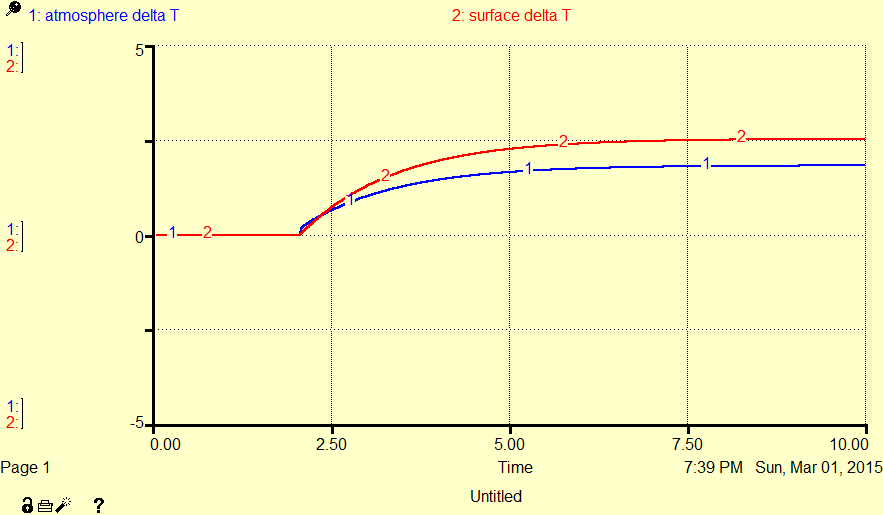
\includegraphics[width=0.9\textwidth]{./p1a.jpg}
\end{figure}
\begin{itemize}
\item Increased solar input from 100 to 103 and held constant
\end{itemize}
}

\frame{
\frametitle{1. Altering the solar input}
\begin{figure}
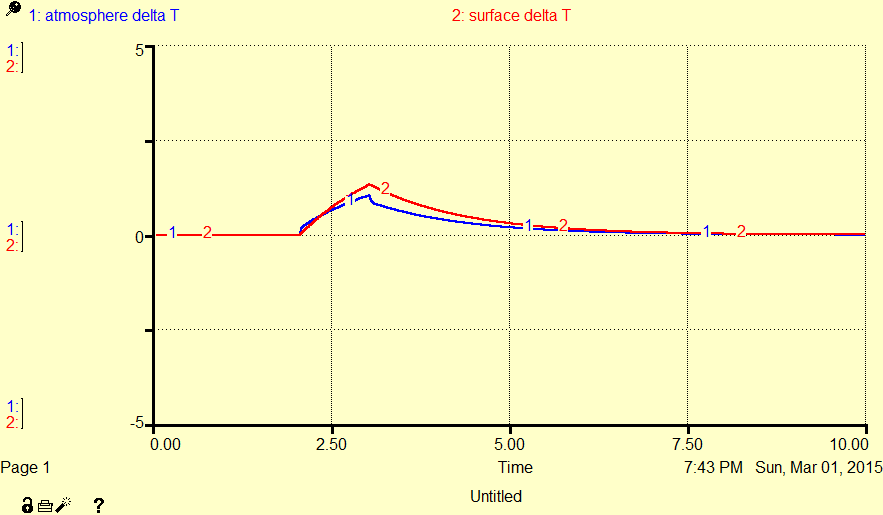
\includegraphics[width=0.9\textwidth]{./p1b.jpg}
\end{figure}
\begin{itemize}
\item Temporarily increased solar input from 100 to 103 for one year
\end{itemize}
}

\frame{
\frametitle{1. Altering the solar input}
\begin{figure}
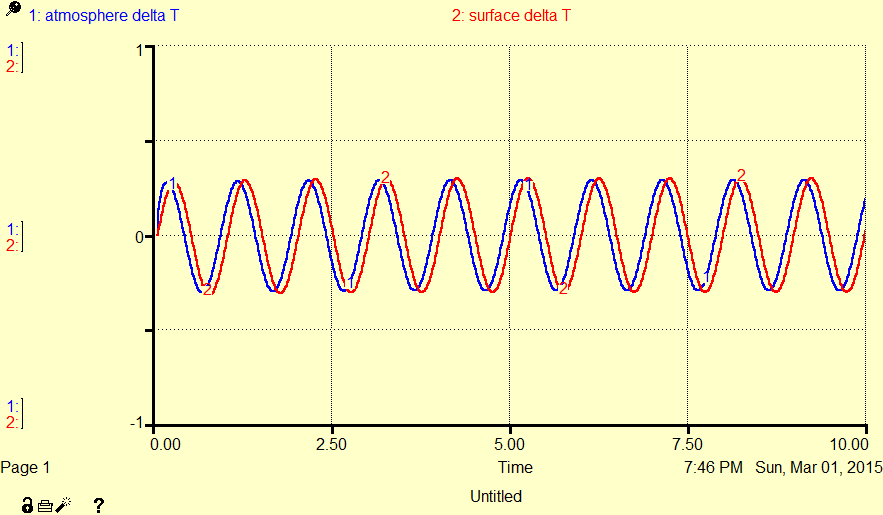
\includegraphics[width=0.9\textwidth]{./p1d.jpg}
\end{figure}
\begin{itemize}
\item Seasonal variability in solar input
\end{itemize}
}

\frame{
\frametitle{2. Altering the cloud cover}
\begin{figure}
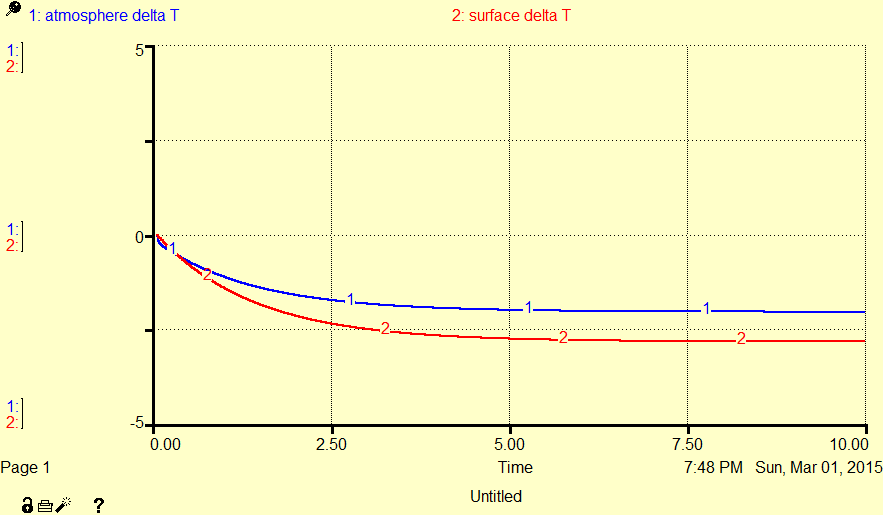
\includegraphics[width=0.9\textwidth]{./p2a.jpg}
\end{figure}
\begin{itemize}
\item Increased cloud cover from 60\% to 65\% $\Rightarrow$ increase in albedo, decrease in absorption of the Earth, and increased greenhouse effect
\end{itemize}
}

\frame{
\frametitle{2. Altering the cloud cover}
\begin{figure}
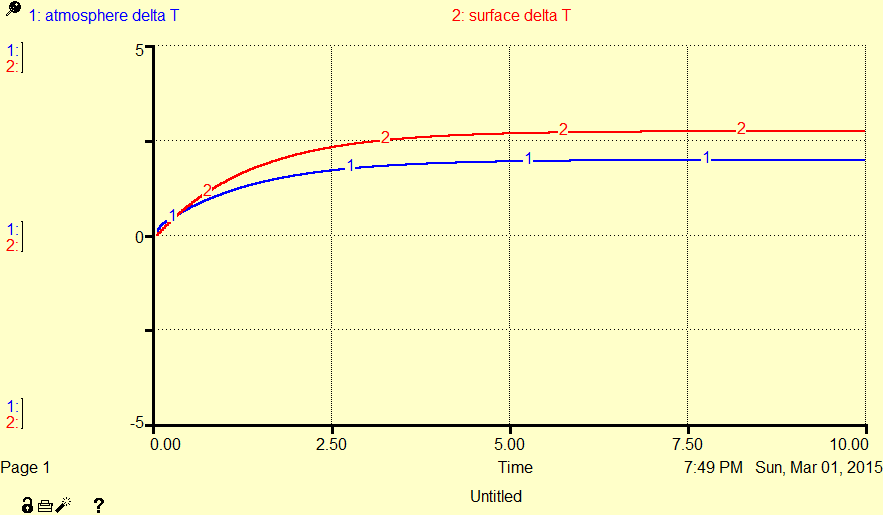
\includegraphics[width=0.9\textwidth]{./p2b.jpg}
\end{figure}
\begin{itemize}
\item decreased cloud cover from 60\% to 55\% $\Rightarrow$ decrease in cloud albedo, decrease in greenhouse effect, and increase in Earth’s absorption
\end{itemize}
}

\frame{
\frametitle{2. Altering the cloud cover}
\begin{figure}
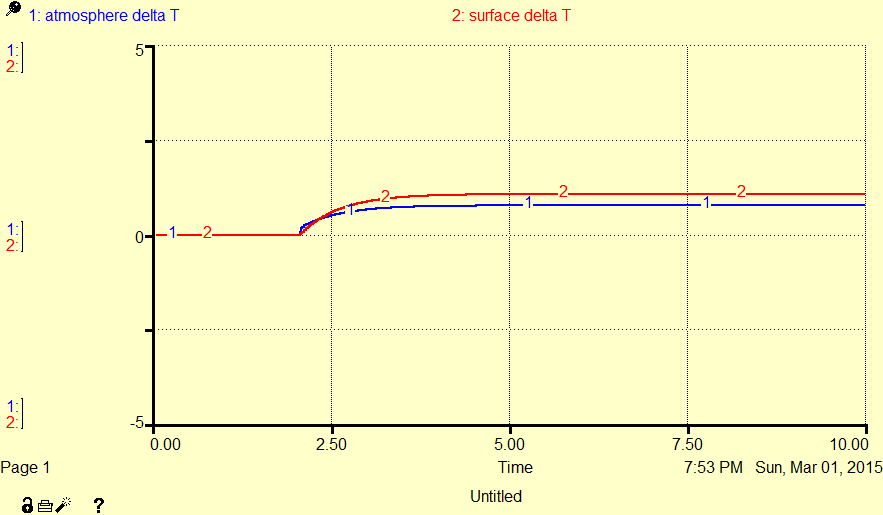
\includegraphics[width=0.9\textwidth]{./p2c.jpg}
\end{figure}
\begin{itemize}
\item cloud cover depends on temperature, change solar steady at 100 then changes to 103 $\Rightarrow$ quicker response and smaller change in temperature
\end{itemize}
}

\frame{
\frametitle{3. Removing the greenhouse effect}
\begin{figure}
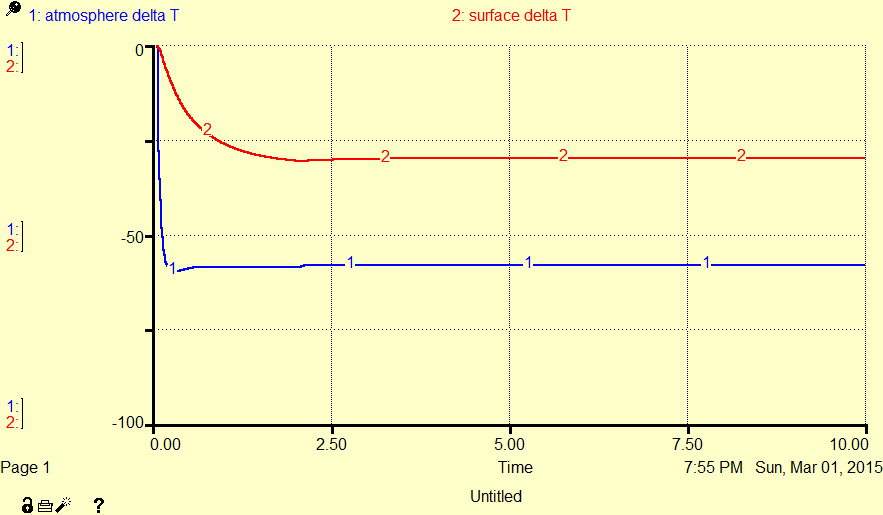
\includegraphics[width=0.9\textwidth]{./p3.jpg}
\end{figure}
}

\frame{
\frametitle{4. Enhancing the greenhouse effect}
\begin{figure}
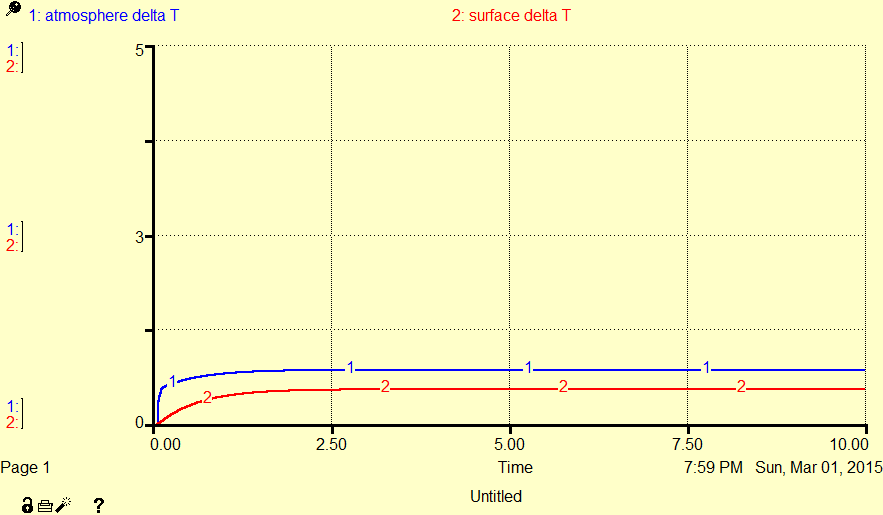
\includegraphics[width=0.9\textwidth]{./p4.jpg}
\end{figure}
}

\frame{
\frametitle{5. Comparing different sources of warming}
\begin{figure}
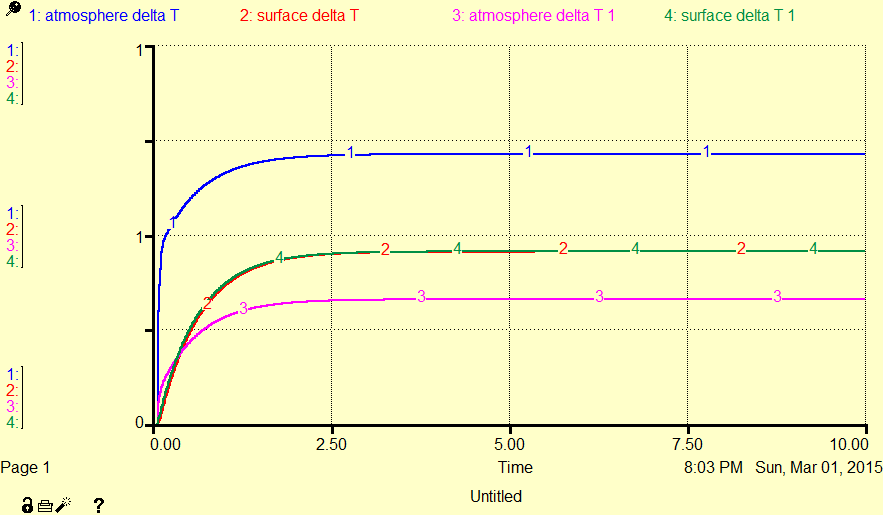
\includegraphics[width=0.9\textwidth]{./p5.jpg}
\end{figure}
\begin{itemize}
\item With the greenhouse effect, the atmosphere responds more strongly than Earth surface (and more quickly in both cases)
\end{itemize}
}

\frame{
\frametitle{Key ideas}
\begin{itemize}
\item System components don't always evolve at the same time, and in some cases may produce systems that are never able to reach a steady state
\item Created a negative feedback by making cloud cover depend on temperature $\rightarrow$ the model still responds to perturbations, but the negative feedback makes it less sensitive to perturbations
\item To understand what is driving changes in a system, often need to look at multiple variables $\rightarrow$ in our case, increased greenhouse gases and increased solar input caused similar changes in the temperature of the Earth's surface, but the former caused a large change in the temperature of the atmosphere was the latter had a smaller impact on the atmosphere
\item Note: important to use the same scale when comparing results from different simulations!
\end{itemize}
}

\end{document}
